
%-------------------------------------------------------------------------------------------
%%%%%%%% PREAMBLE
%-------------------------------------------------------------------------------------------
\documentclass[11pt]{article}

% Load packages
\usepackage[T1]{fontenc}

\usepackage{aeguill}
\usepackage{fancyhdr, amssymb, amsmath, geometry,setspace,lastpage,pdflscape}
\usepackage[pdftex]{graphicx,color}
\definecolor{dkblue}{rgb}{0,0.08,0.45}
\usepackage[pdftex]{hyperref}
\hypersetup{colorlinks}%
%citecolor=black,%
%filecolor=black,%
%linkcolor=black,%
%urlcolor=black}

%\usepackage{lmodern}
\usepackage{helvet}
\renewcommand{\familydefault}{\sfdefault}

% Page Setup
\geometry{ top = 1in, bottom = 1in , left=1in, right=1in}
\pagestyle{empty}
\lhead{}
\chead{}
\rhead{}
\lfoot{}
\cfoot{\footnotesize \thepage  { /}  \pageref{LastPage}}
\rfoot{}

% Paragraph Setup
\setlength{\parskip}{\baselineskip}%
\setlength{\parindent}{0pt}%

% Title Information
\title{}
\author{}
\date{}

%-------------------------------------------------------------------------------------------
%%%%%%%% DOCUMENT BEGINS HERE
%-------------------------------------------------------------------------------------------
\begin{document}

%\begin{center}
%{\Large Main Text Figures}
%\end{center}
%\vspace{50pt}


\renewcommand{\figurename}{Fig.}

%-------------------------------------------------------------------------------------------
% Figure 1 - Garki results
%-------------------------------------------------------------------------------------------

%\begin{landscape}
\begin{figure}[htbp]
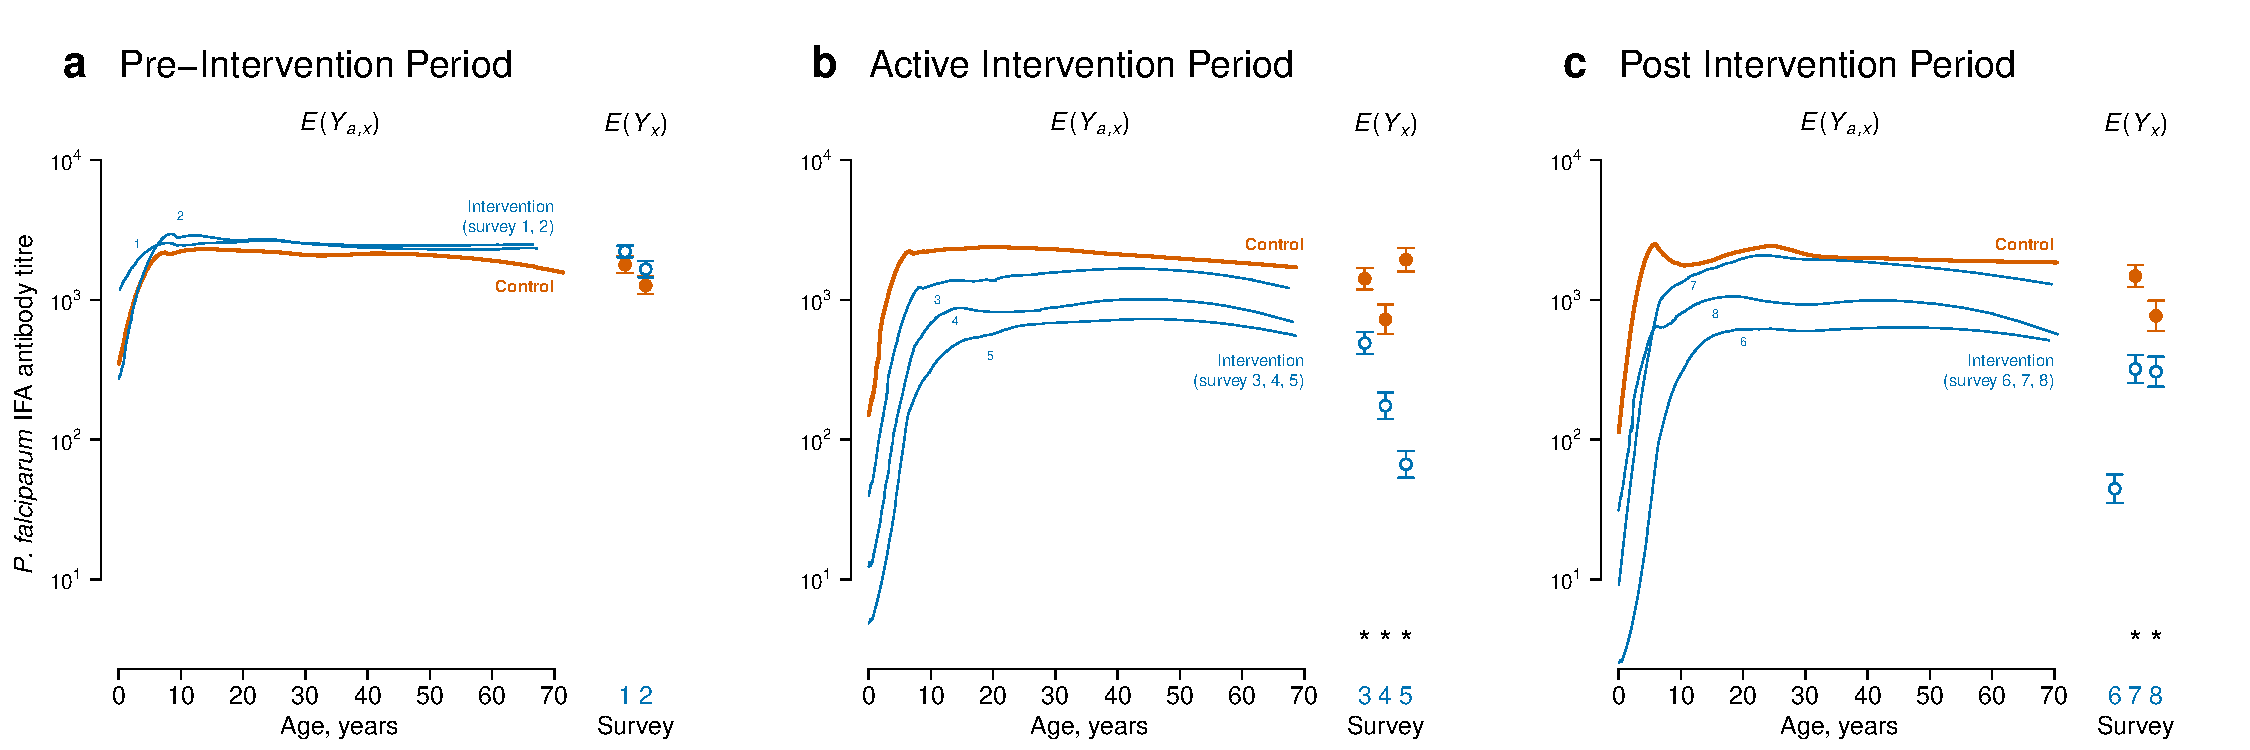
\includegraphics[width=\textwidth]{/users/benarnold/dropbox/articles/antibody-curves/results/figs/garki-antibody-curves-IFAPf.pdf} \\
\hspace*{\fill} 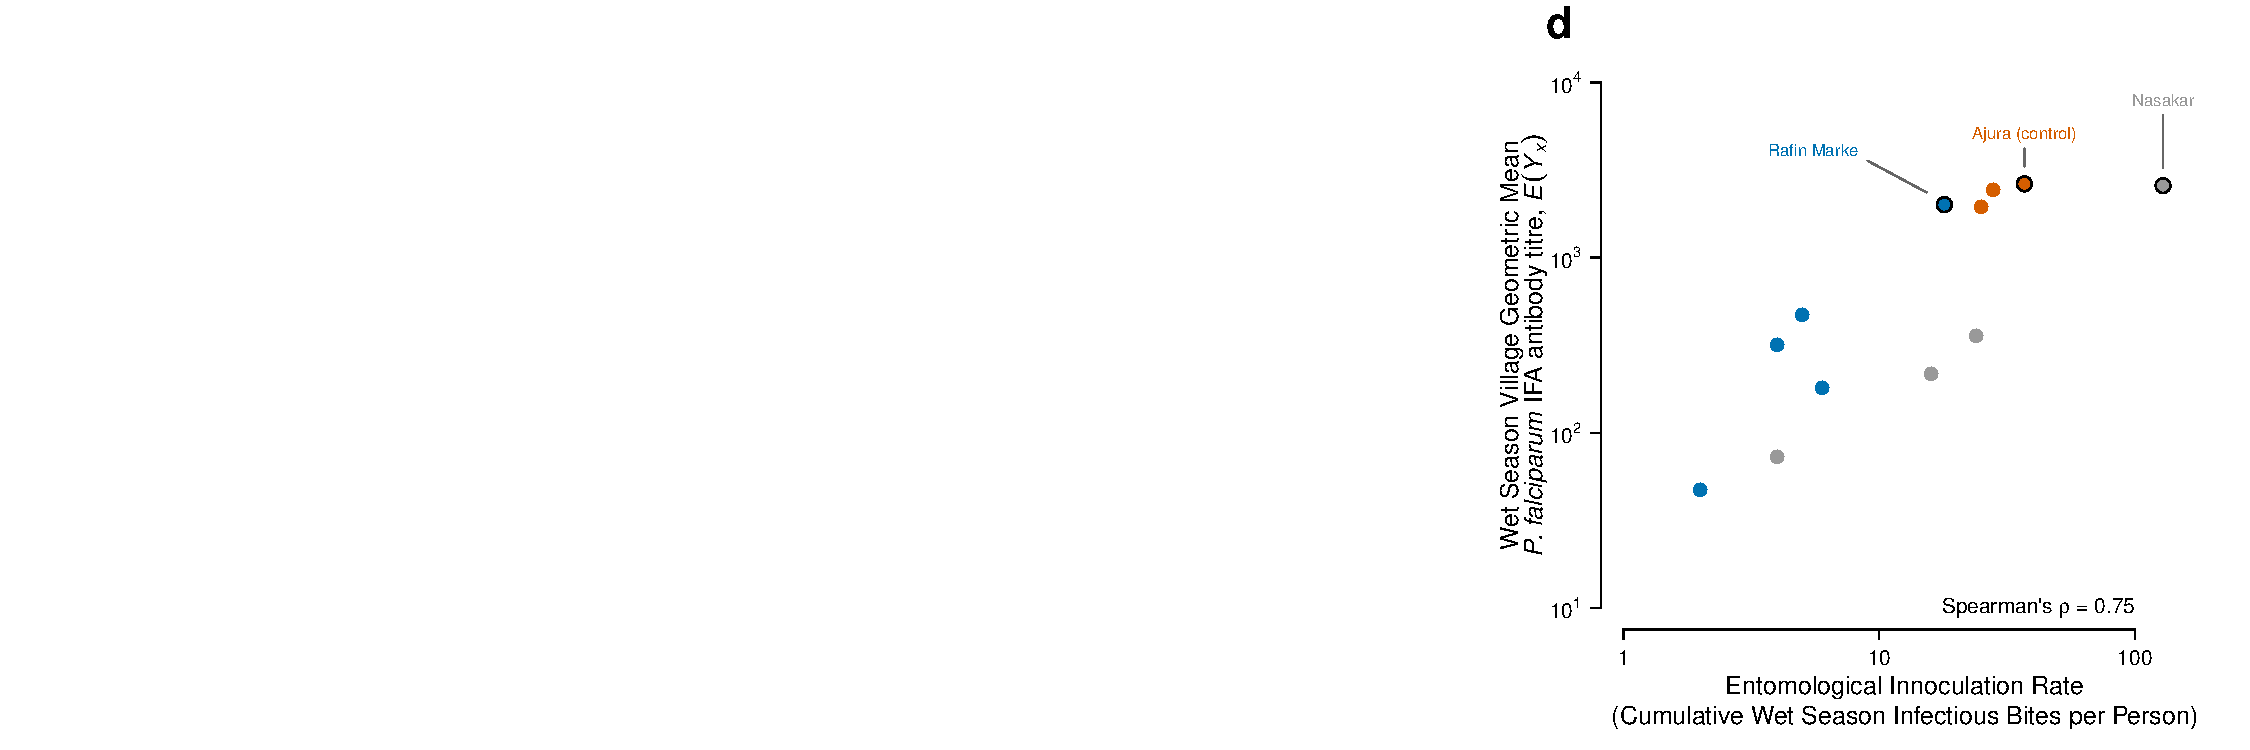
\includegraphics[width=0.33\textwidth]{/users/benarnold/dropbox/articles/antibody-curves/results/figs/garki-IFAPf-EIR.pdf} 

\begin{center}
\begin{minipage}{\textwidth}
\caption{Shifts in the \textit{Plasmodium falciparum} age-antibody curve measure changes in malaria transmission due to intervention in the Garki Project, Nigeria (1970-1976). The intervention included a combination of insecticide spraying and mass drug administration of surfanene-pyrimethamine in 1972-1973. Antibody response measured with the IgG indirect fluorescent antibody (IFA) test for \textit{P. falciparum}. \textbf{a}, pre-intervention period wet and dry seasons measures (survey rounds 1-2); \textbf{b}, active intervention period (survey rounds 3-5, at 20, 50, and 70 weeks following the start of intervention); \textbf{c}, post-intervention period (survey rounds 6-8 at 20, 40, and 90 weeks following the end of the intervention).  Age-antibody curves, $E(Y_{a,x})$ by age ($a$) and intervention group ($x$), were fit using antibody responses in individuals (N=6,024 total measurements, with 459 - 551 measurements per curve) using a nonparametric ensemble machine learning algorithm (Online Methods). Control measurements were combined across survey rounds within each period when plotting the curves to facilitate visual comparison of shifts in transmission intensity between surveys. Age-adjusted geometric means by intervention group, $E(Y_x)$, provide summary differences between curves at each survey round. Error bars show 95\% confidence intervals for the age-adjusted geometric means and asterisks indicate $P\leq0.01$ (Bonferroni corrected) for differences between control and intervention groups. Control villages were not measured in survey 6. \textbf{d}, Village-level, age-adjusted geometric mean \textit{P. falciparum} IFA titres, $E(Y_x)$, versus wet season entomological inoculation rate (EIR) in the three study villages with both entomological and serological measurements. Ajura was a control village (no treatment) while Rafine Marke and Nasakar were intervention villages.  The circled and labeled points are from the 1971 wet season (pre-intervention) and other points represent wet seasons for 1972-73 (Ajura) or 1972-75 (Rafine Marke and Nasakar). A single data point outside the figure range is not shown (Nasakar 1972, EIR value = 0, $E(Y_x) = 10^{3.0591}$), but was included in the Spearman rank correlation estimate.   }
\label{fig:garki}
\end{minipage}
\end{center}
\end{figure}
%\end{landscape}
% note: timing of surveys estimated from Figs 1, 2 and 4 of Cornille-Broger 1978 Bull World Health Org  56 (4): 579-600


%-------------------------------------------------------------------------------------------
% Figure 2 - Garki wet and dry season results
%-------------------------------------------------------------------------------------------
\begin{figure}[htbp]
\begin{center}
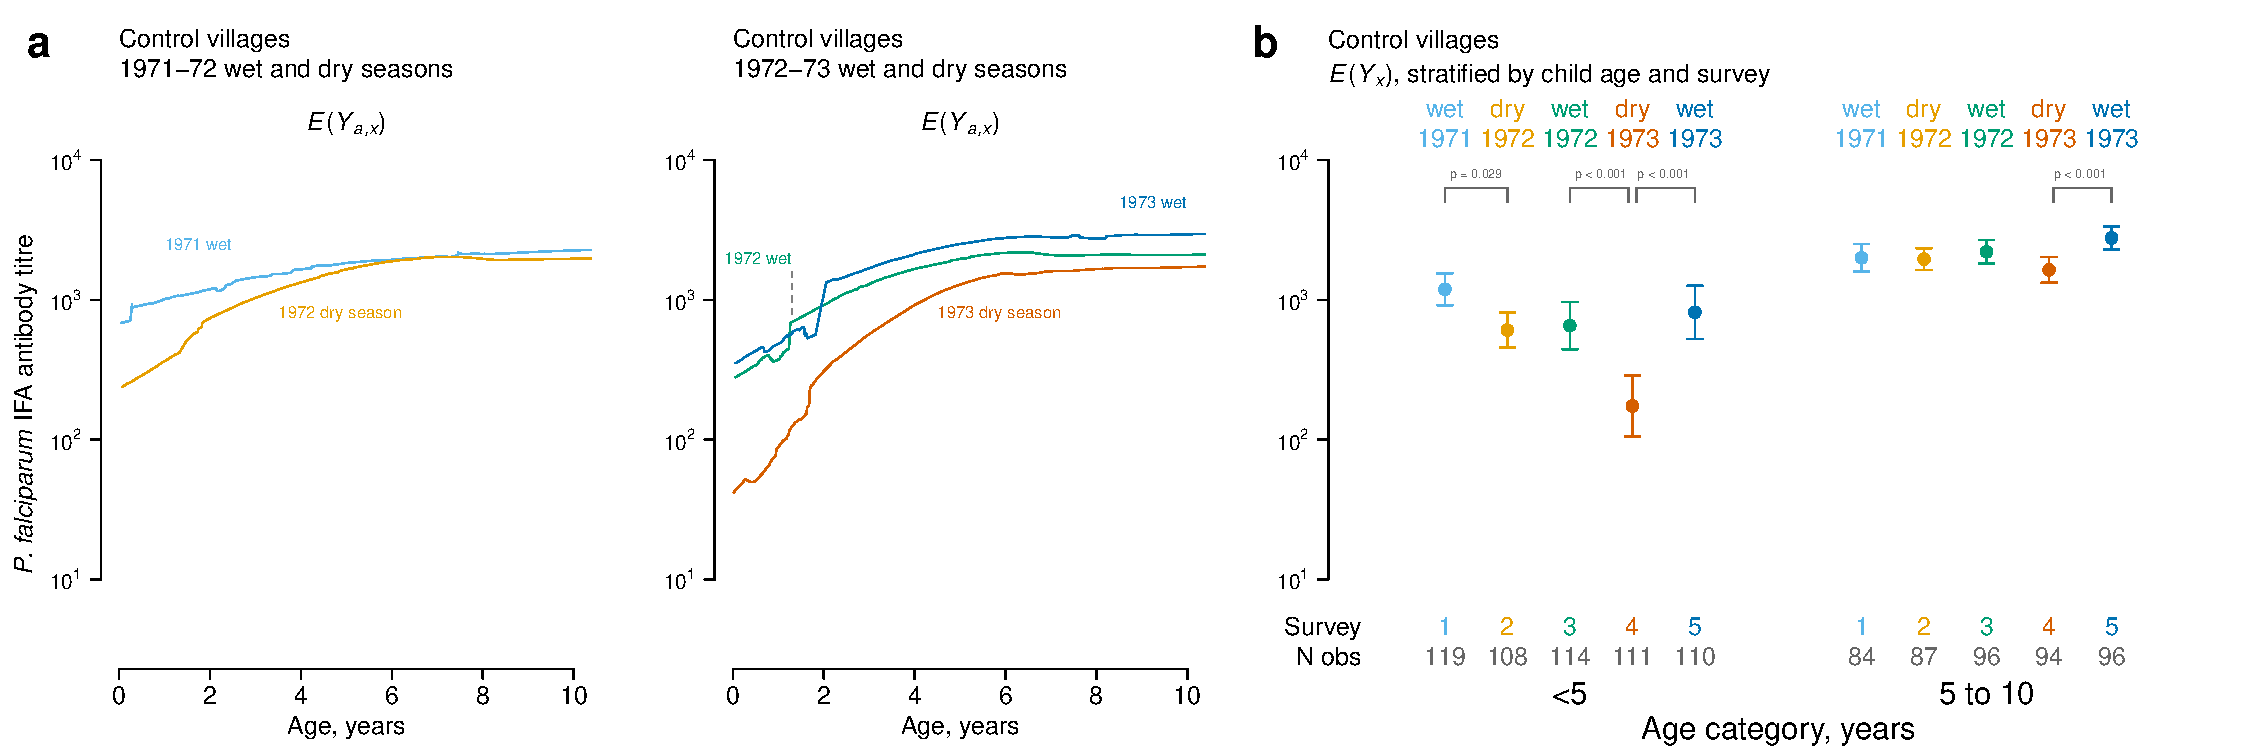
\includegraphics[width=\textwidth]{/users/benarnold/dropbox/articles/antibody-curves/results/figs/garki-wet-dry-analysis.pdf}
\begin{minipage}{\textwidth}
\caption{Higher sensitivity among children <5 to seasonal changes in \textit{Plasmodium falciparum} transmission as depicted by age-antibody curves estimated within control villages in the Garki Project, Nigeria (1970-1976). Antibody response measured with the IgG indirect fluorescent antibody (IFA) test for \textit{P. falciparum}.  \textbf{a}, age-antibody curves, $E(Y_{a,x})$ by age ($a$) and season ($x$), were fit using antibody responses in individuals as described in Fig 1. \textbf{b}, Age-adjusted geometric means by age category and season, $E(Y_x)$, summarize the curves. Error bars show 95\% confidence intervals and \textit{P}-values mark significant differences (Bonferroni corrected) between adjacent seasons.  }
\label{fig:garkiwetdry}
\end{minipage}
\end{center}
\end{figure}


%-------------------------------------------------------------------------------------------
% Figure 3 - Mauke results
%-------------------------------------------------------------------------------------------
\begin{figure}[htbp]
\begin{center}
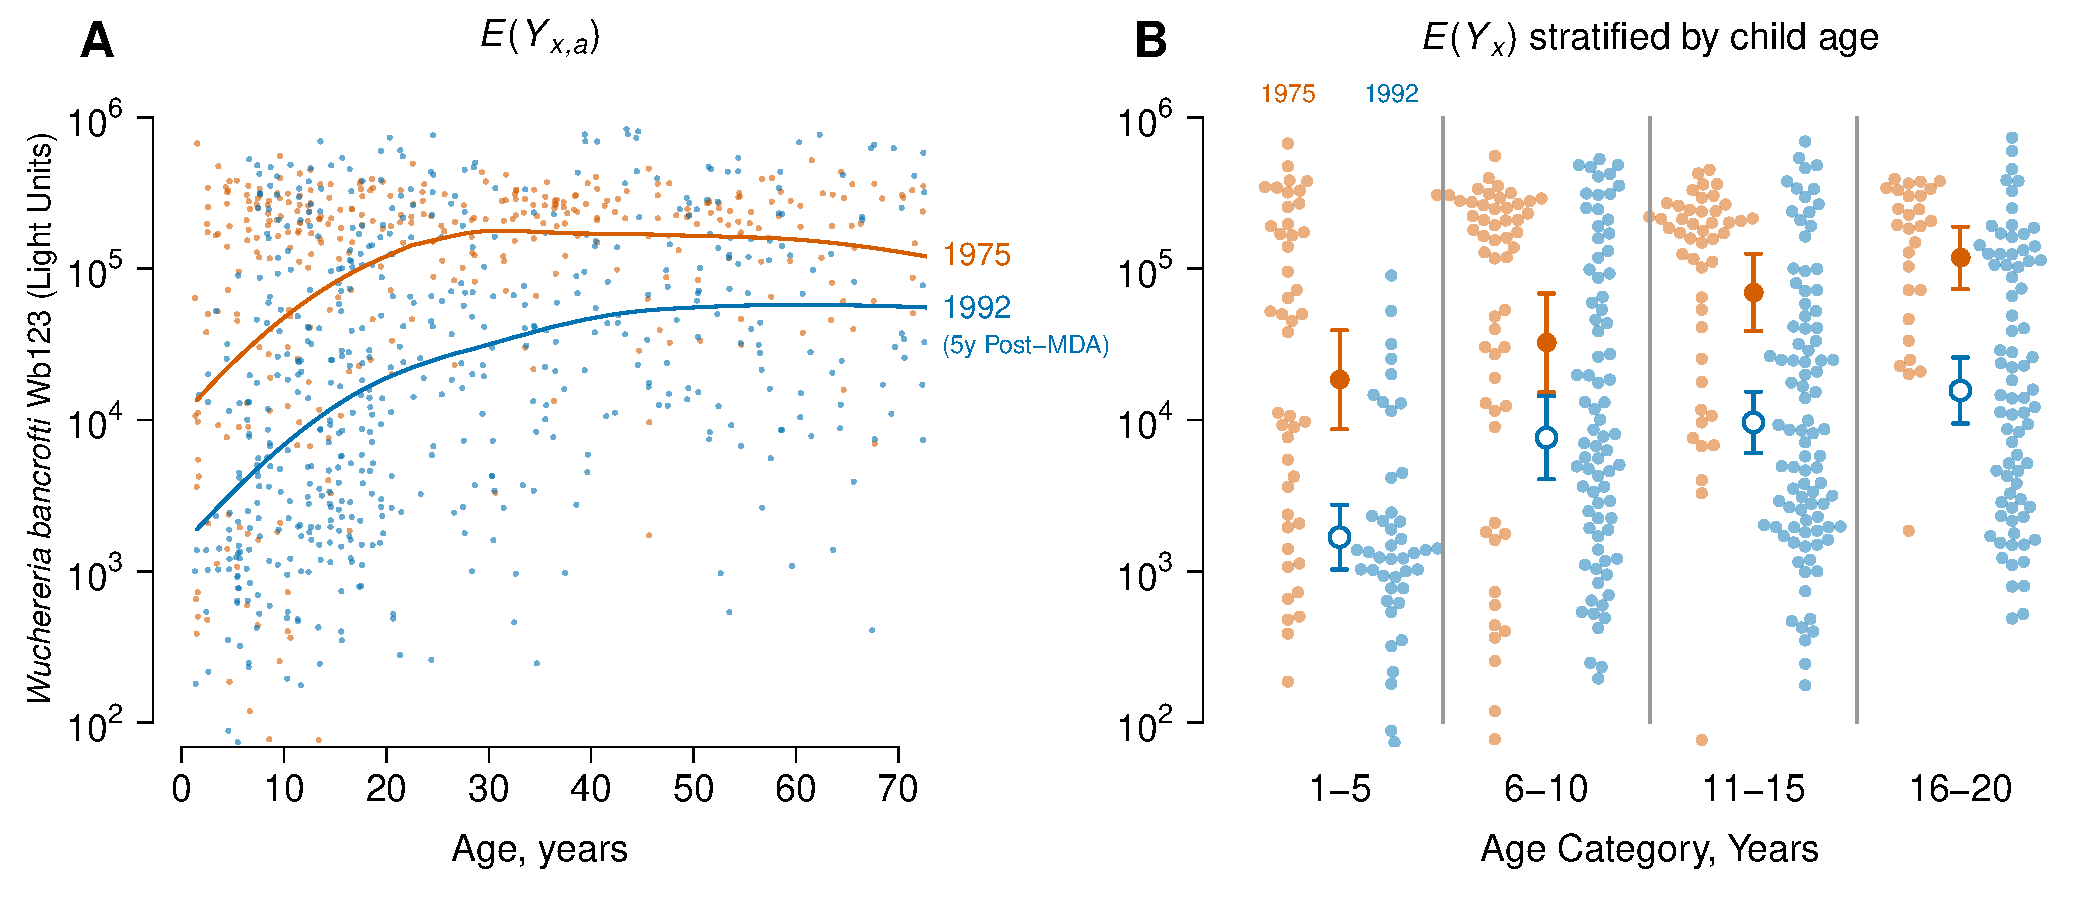
\includegraphics[width=\textwidth]{/users/benarnold/dropbox/articles/antibody-curves/results/figs/mauke-Wb123-analysis.pdf} \\
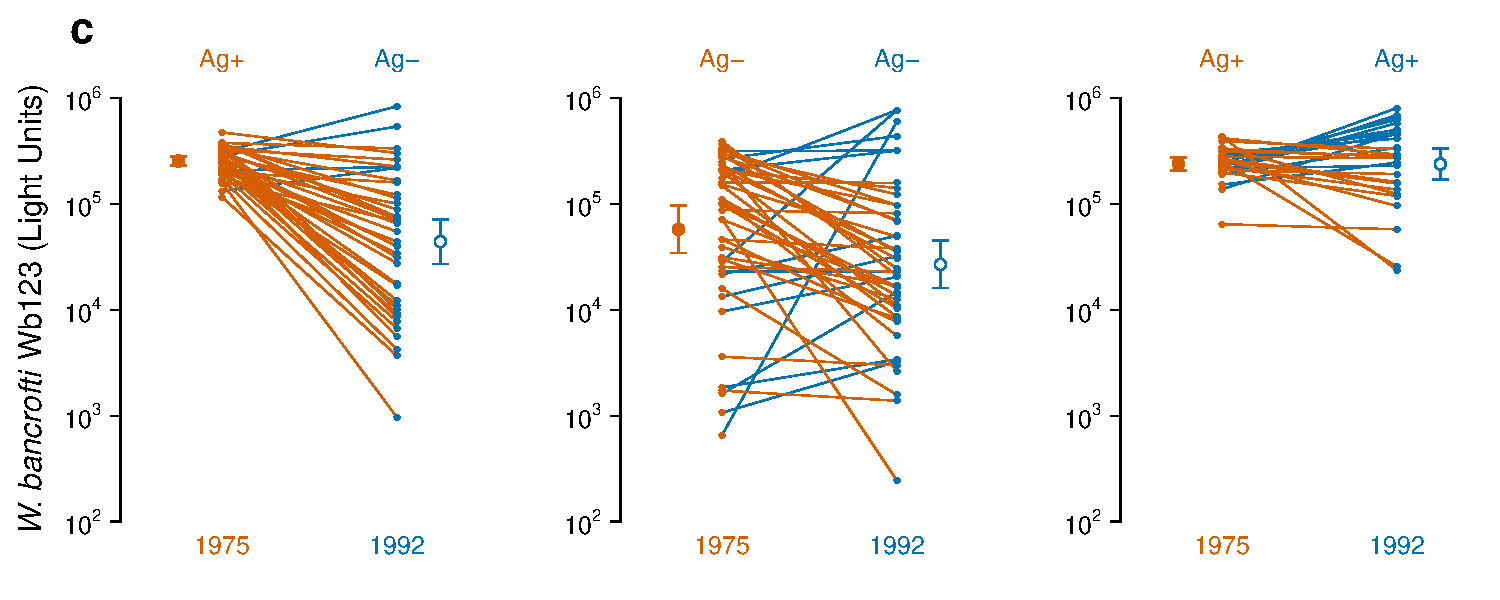
\includegraphics[width=\textwidth]{/users/benarnold/dropbox/articles/antibody-curves/results/figs/mauke-Wb123-long.pdf}
\begin{minipage}{\textwidth}
\caption{A shift in the age-antibody curve measures a reduction in transmission intensity of \textit{Wuchereria bancrofti} due to mass drug administration (MDA) on Mauke Island.  IgG antibody response to the Wb123 antigen for \textit{W. bancrofti} measured in blood specimens from residents in 1975 (N=362) before MDA and again in 1992 (N=553), five years following a single, island-wide MDA with diethylcarbamazine. Geometric mean antibody levels $E(Y_{a,x})$ by age ($a$) and survey year ($x$); individual antibody responses (points) are shown along with summary curves fit with a nonparametric ensemble machine learning algorithm (Online Methods). \textbf{b}, Age-adjusted geometric mean antibody response $E(Y_{x})$ and 95\% confidence intervals before (1975) and five years after (1992) MDA, stratified by 5 year age category (all differences significant at $P\leq0.01$ after Bonferroni correction). \textbf{c}, Wb123 antibody response in 1975 and 1992 stratified by the presence of circulating filarial antigens (Ag) at each measurement in the subsample of 112 individuals who were measured at both time points (two individuals not shown were Ag- in 1975 and Ag+ in 1992), along with age-adjusted geometric means, $E(Y_{x})$, and 95\% confidence intervals. Differences between means are significant (Bonferroni corrected $P\leq0.02$) except for the Ag+/Ag+ group. Individual trajectories are colored by the higher of the two measurements: decreases are orange, increases are blue. }
\label{fig:mauke}
\end{minipage}
\end{center}
\end{figure}

%-------------------------------------------------------------------------------------------
% Figure 4 - Enterics
%-------------------------------------------------------------------------------------------

\begin{figure}[htbp]
\begin{center}
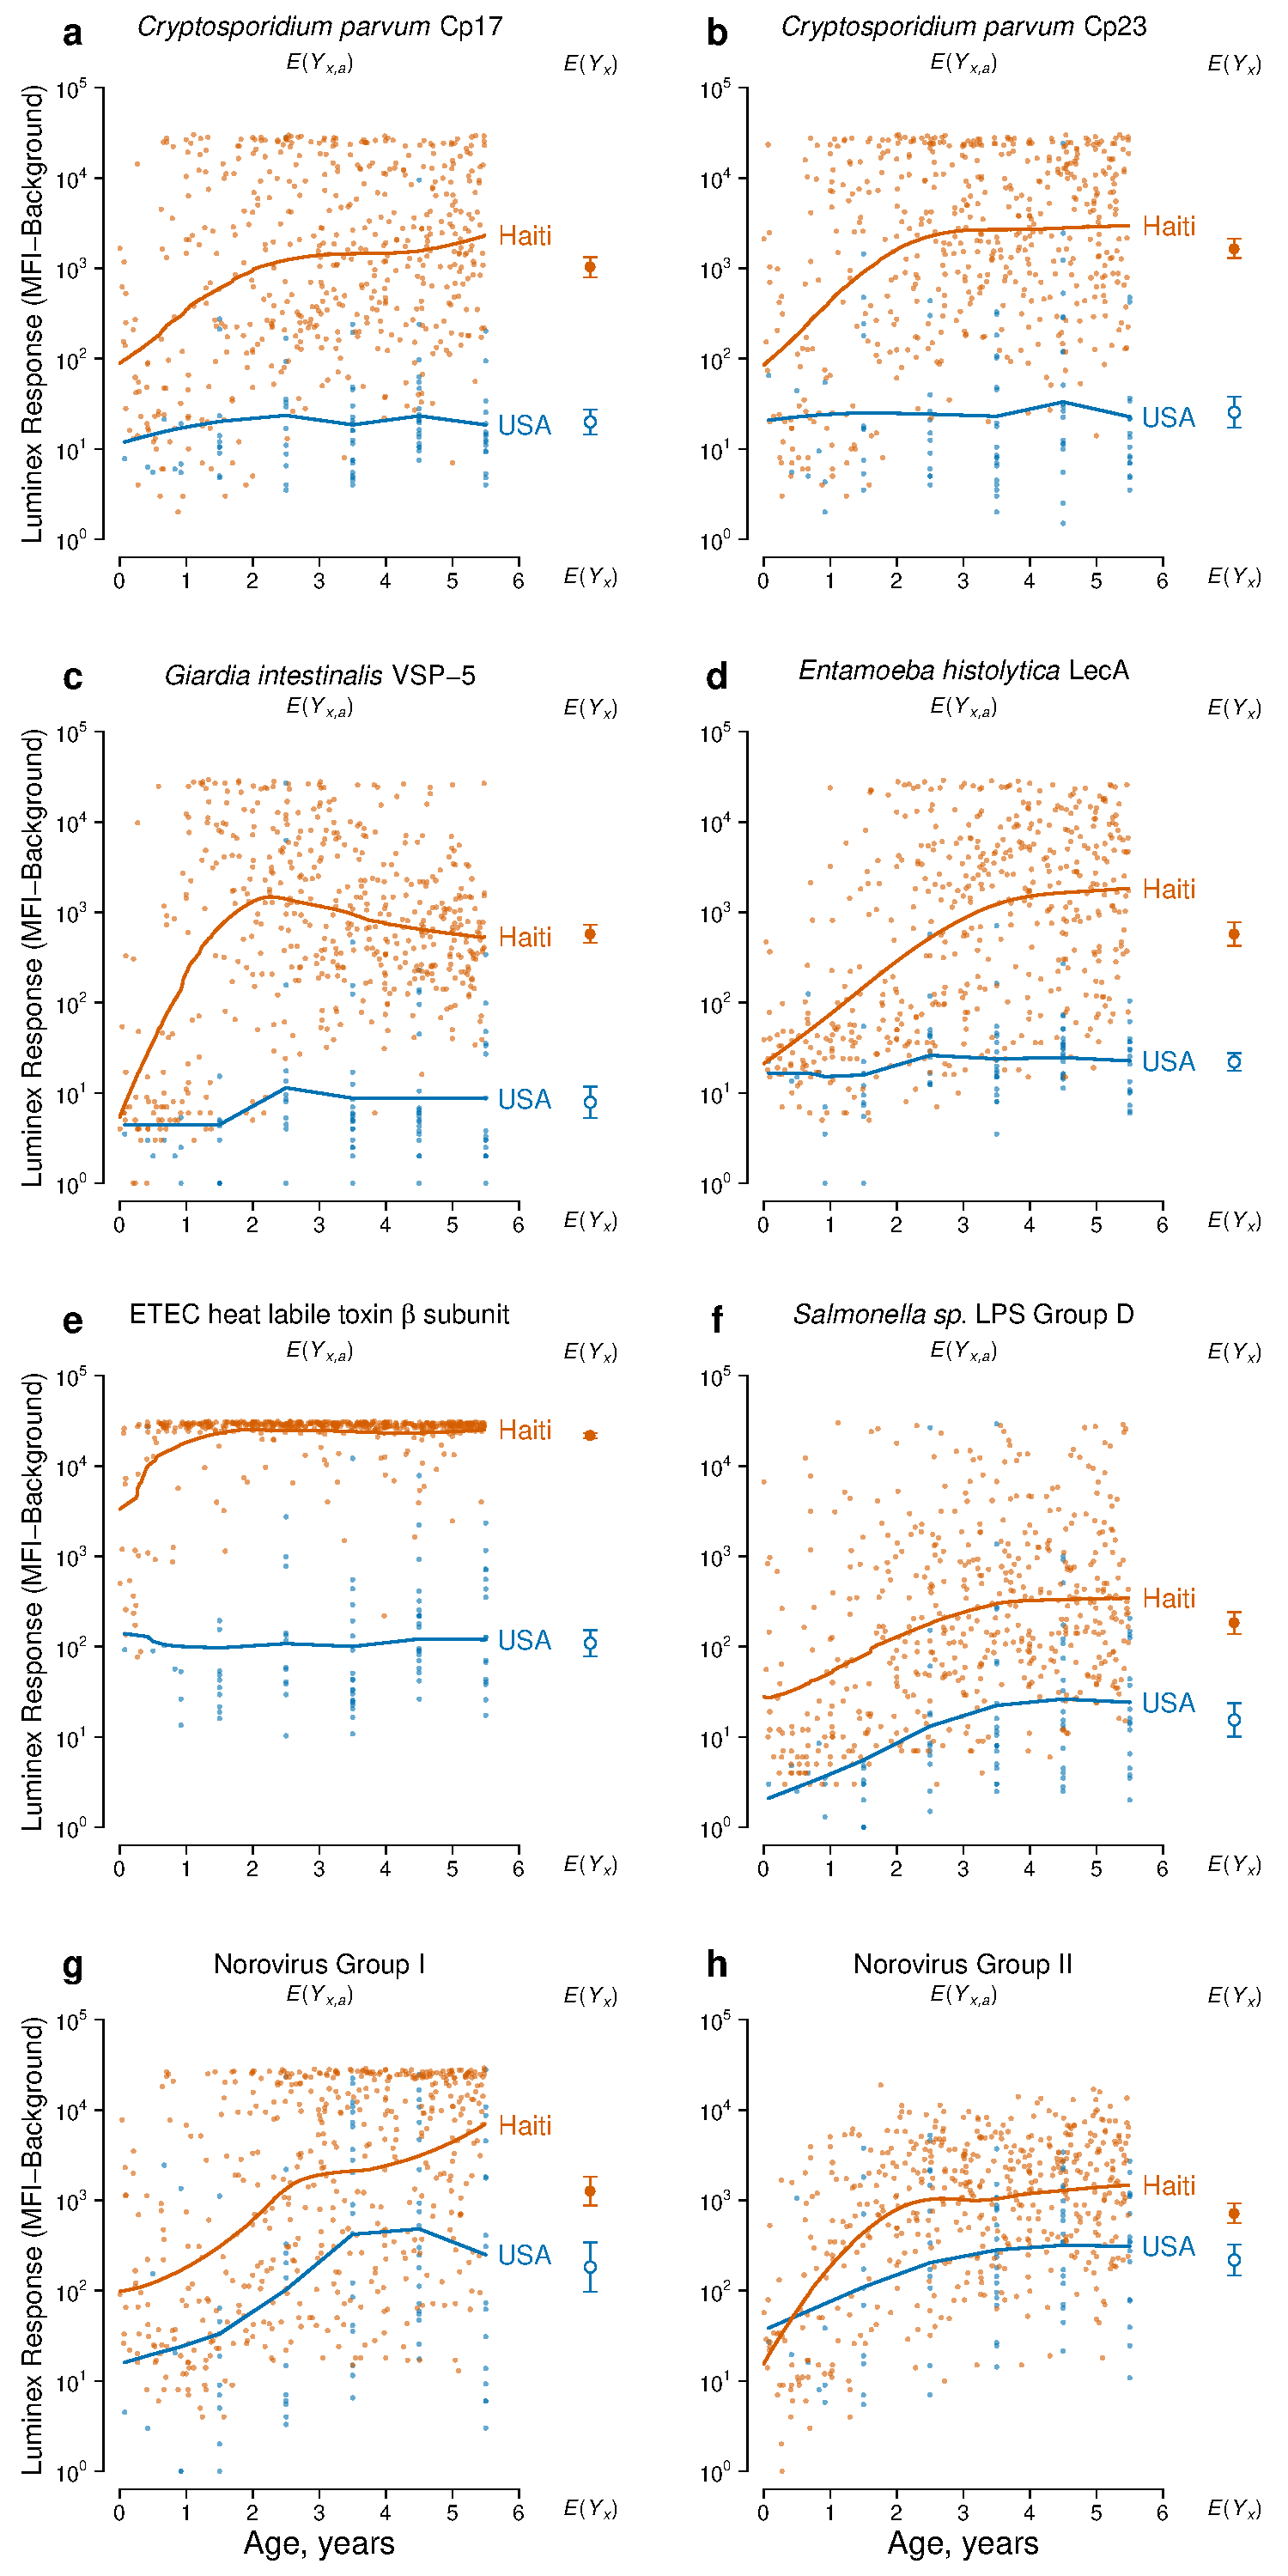
\includegraphics[width=0.7\textwidth]{/users/benarnold/dropbox/articles/antibody-curves/results/figs/haiti2-USA-enterics-SL-curves.pdf}
\begin{minipage}{\textwidth}
\caption{caption on the next page}
\label{fig:enterics}
\end{minipage}
\end{center}
\end{figure}

\clearpage
Fig 4: Differences in enteric pathogen transmission between children in Leogane, Haiti (N=511) and the United States (USA) (N=86) measured by age-antibody curves. Antibody response measured as median fluorescence intensity (MFI) minus background in multiplex bead assays on the Luminex platform. In each panel, individual antibody responses (points) are shown along with age-specific summary curves, $E(Y_{a,x})$, by age ($a$) and country ($x$), fit with an ensemble machine learning algorithm (Online Methods). Each panel also includes the geometric mean by country, $E(Y_{x})$, with error bars indicating 95\% confidence intervals (all differences significant at $P\leq0.01$ after Bonferroni correction).
\textbf{a.} \textit{Cryptosporidium parvum} recombinant 17-kDa antigen;
\textbf{b.} \textit{Cryptosporidium parvum} recombinant 27-kDa antigen;
\textbf{c.} \textit{Giardia intestinalis} variant-specific surface protein-5 (VSP-5);
\textbf{d.} \textit{Entamoeba histolytica} lectin adhesion molecule (LecA);
\textbf{e.} enterotoxigenic \textit{Escherichia coli} (ETEC) heat labile toxin $\beta$ subunit;
\textbf{f.} \textit{Salmonella spp.} lipopolysaccharide (LPS) Group B;
\textbf{g.} Norovirus Group I.4;
\textbf{h.} Norovirus Group II.4 New Orleans.

%-------------------------------------------------------------------------------------------
% Supporting information figures
%-------------------------------------------------------------------------------------------
\clearpage
\begin{center}
{\Large Supplementary Figures}
\end{center}
\vspace{50pt}

% set Table and Figure Numbering to have an "S" prefix
%\renewcommand{\thetable}{S\arabic{table}}
\renewcommand{\figurename}{Supplementary Fig.}
\setcounter{figure}{0} 
%\renewcommand{\thefigure}{S\arabic{figure}}



%-------------------------------------------------------------------------------------------
% Figure S1 - Garki village level results
%-------------------------------------------------------------------------------------------
\clearpage
\begin{figure}[htbp]
\begin{center}
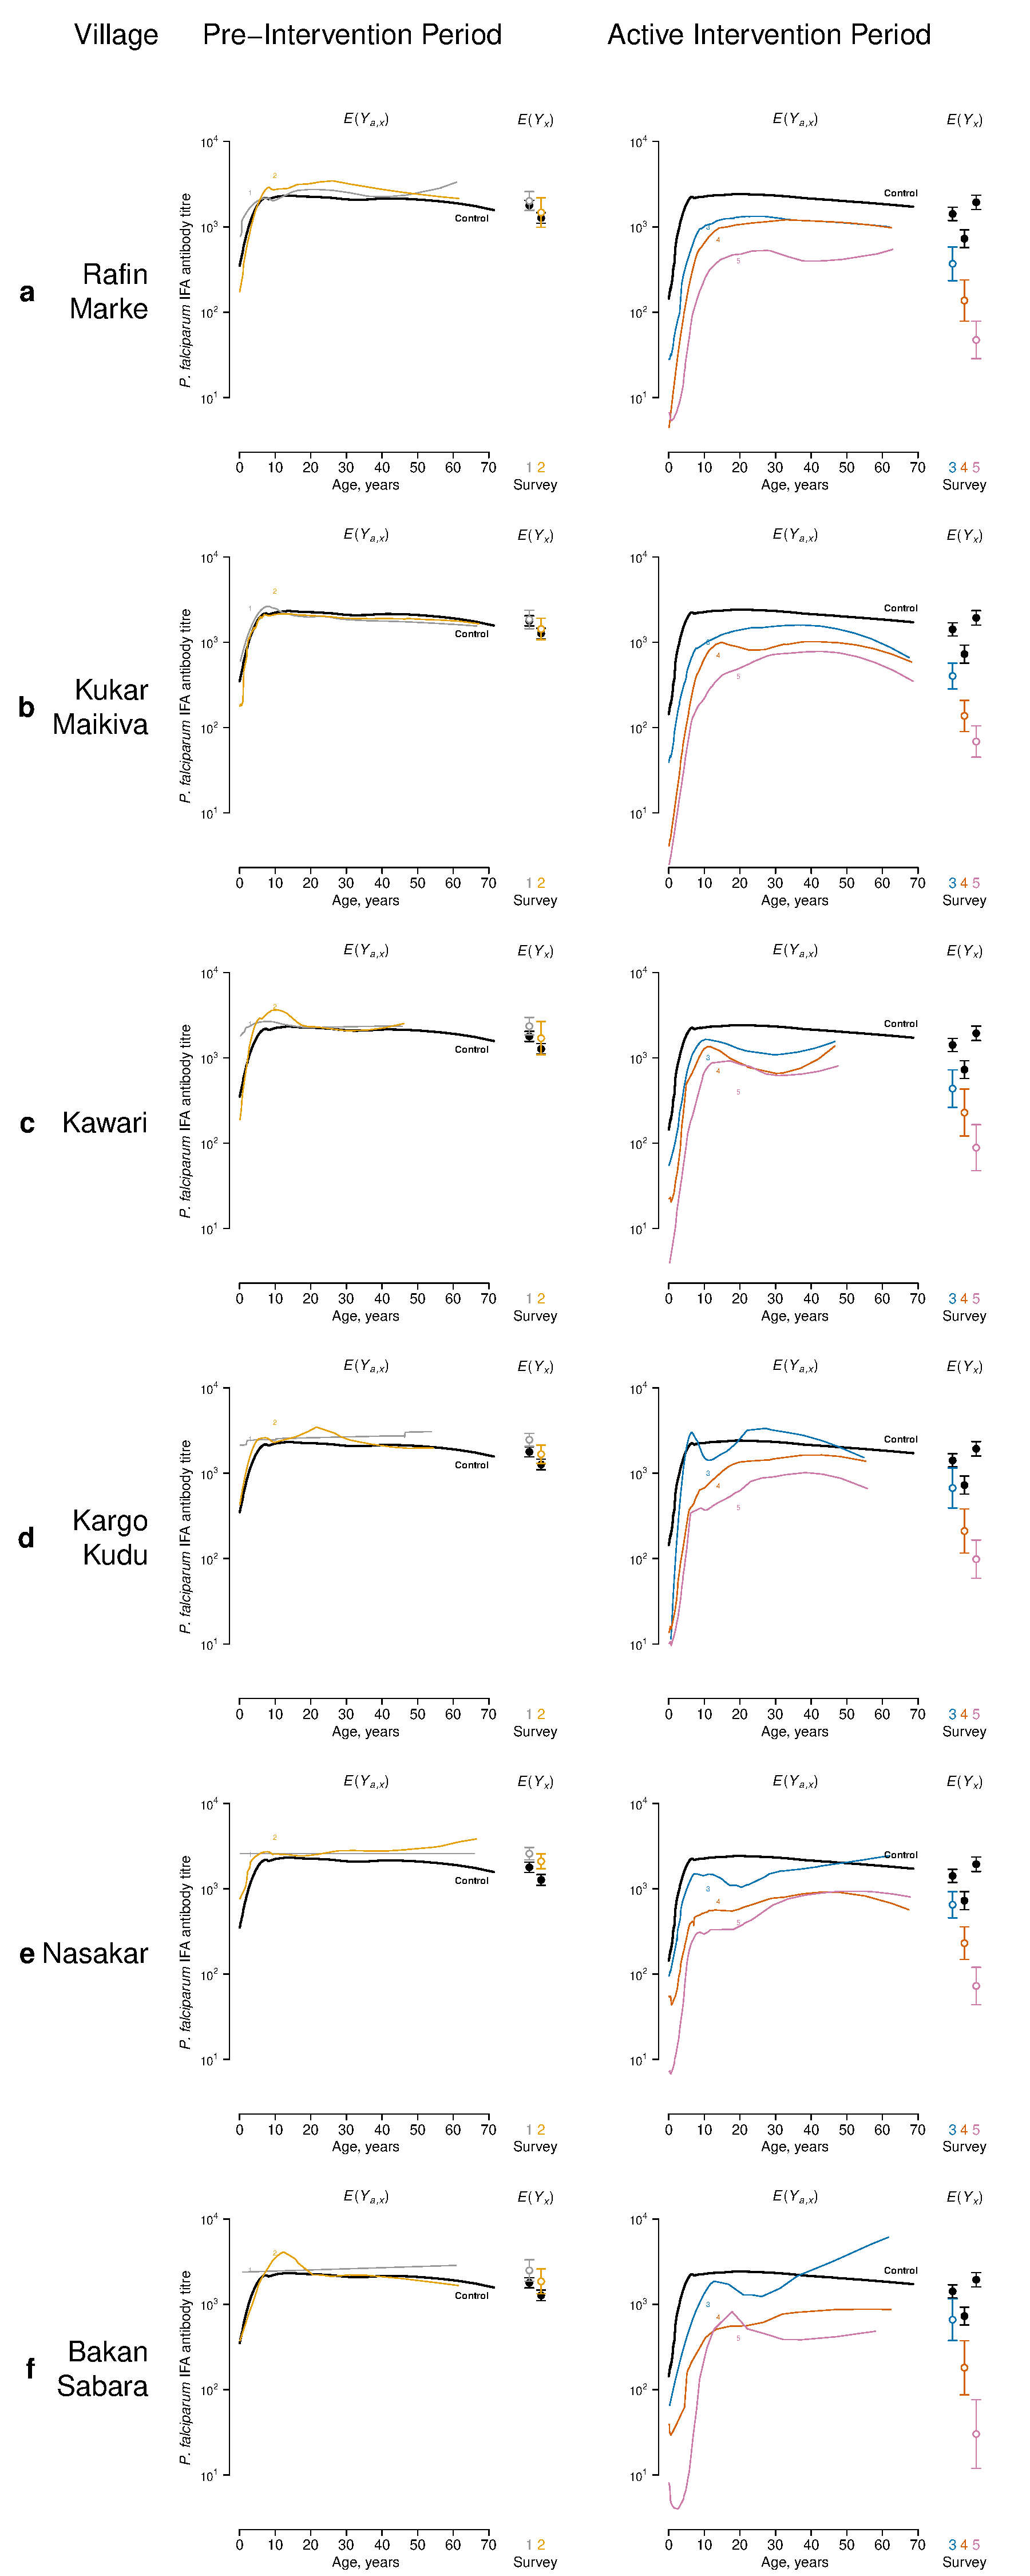
\includegraphics[width=0.6\textwidth]{/users/benarnold/dropbox/articles/antibody-curves/results/figs/garki-IFAPf-by-village.pdf}
\begin{minipage}{\textwidth}
\caption{Caption on the following page.}
\label{fig:garkiVillageEy}
\end{minipage}
\end{center}
\end{figure}
\clearpage
Supplementary Fig. 1: \textit{Plasmodium falciparum} age-antibody curves estimated separately for each intervention village (\textbf{a-f}) measure reductions in malaria transmission due to intervention in the Garki Project, Nigeria (1970-1976).  Antibody response measured with the indirect fluorescent antibody (IFA) test for \textit{P. falciparum}. Panels for each intervention village summarize pre-intervention period wet and dry seasons measures (survey rounds 1-2) and active intervention period (survey rounds 3-5, at 20, 50, and 70 weeks following the start of intervention).  Age-antibody curves, $E(Y_{a,x})$ by age ($a$) and group ($x$), were estimated nonparametrically from quantitative antibody responses in individuals using an ensemble machine learning algorithm (Online Methods). Age-adjusted geometric means by group, $E(Y_x)$, provide summary differences between curves at each survey round. Error bars show 95\% confidence intervals for the age-adjusted geometric means. Each panel includes the same results for the two control villages (black) for comparison.  Control measurements were combined across survey rounds within each period when plotting the curves to facilitate visual comparison of shifts in transmission intensity between surveys. 


%-------------------------------------------------------------------------------------------
% Figure S2 - Miton E(Yx,a) and E(Yx) estimates
%-------------------------------------------------------------------------------------------
\clearpage
\begin{figure}[htbp]
\begin{center}
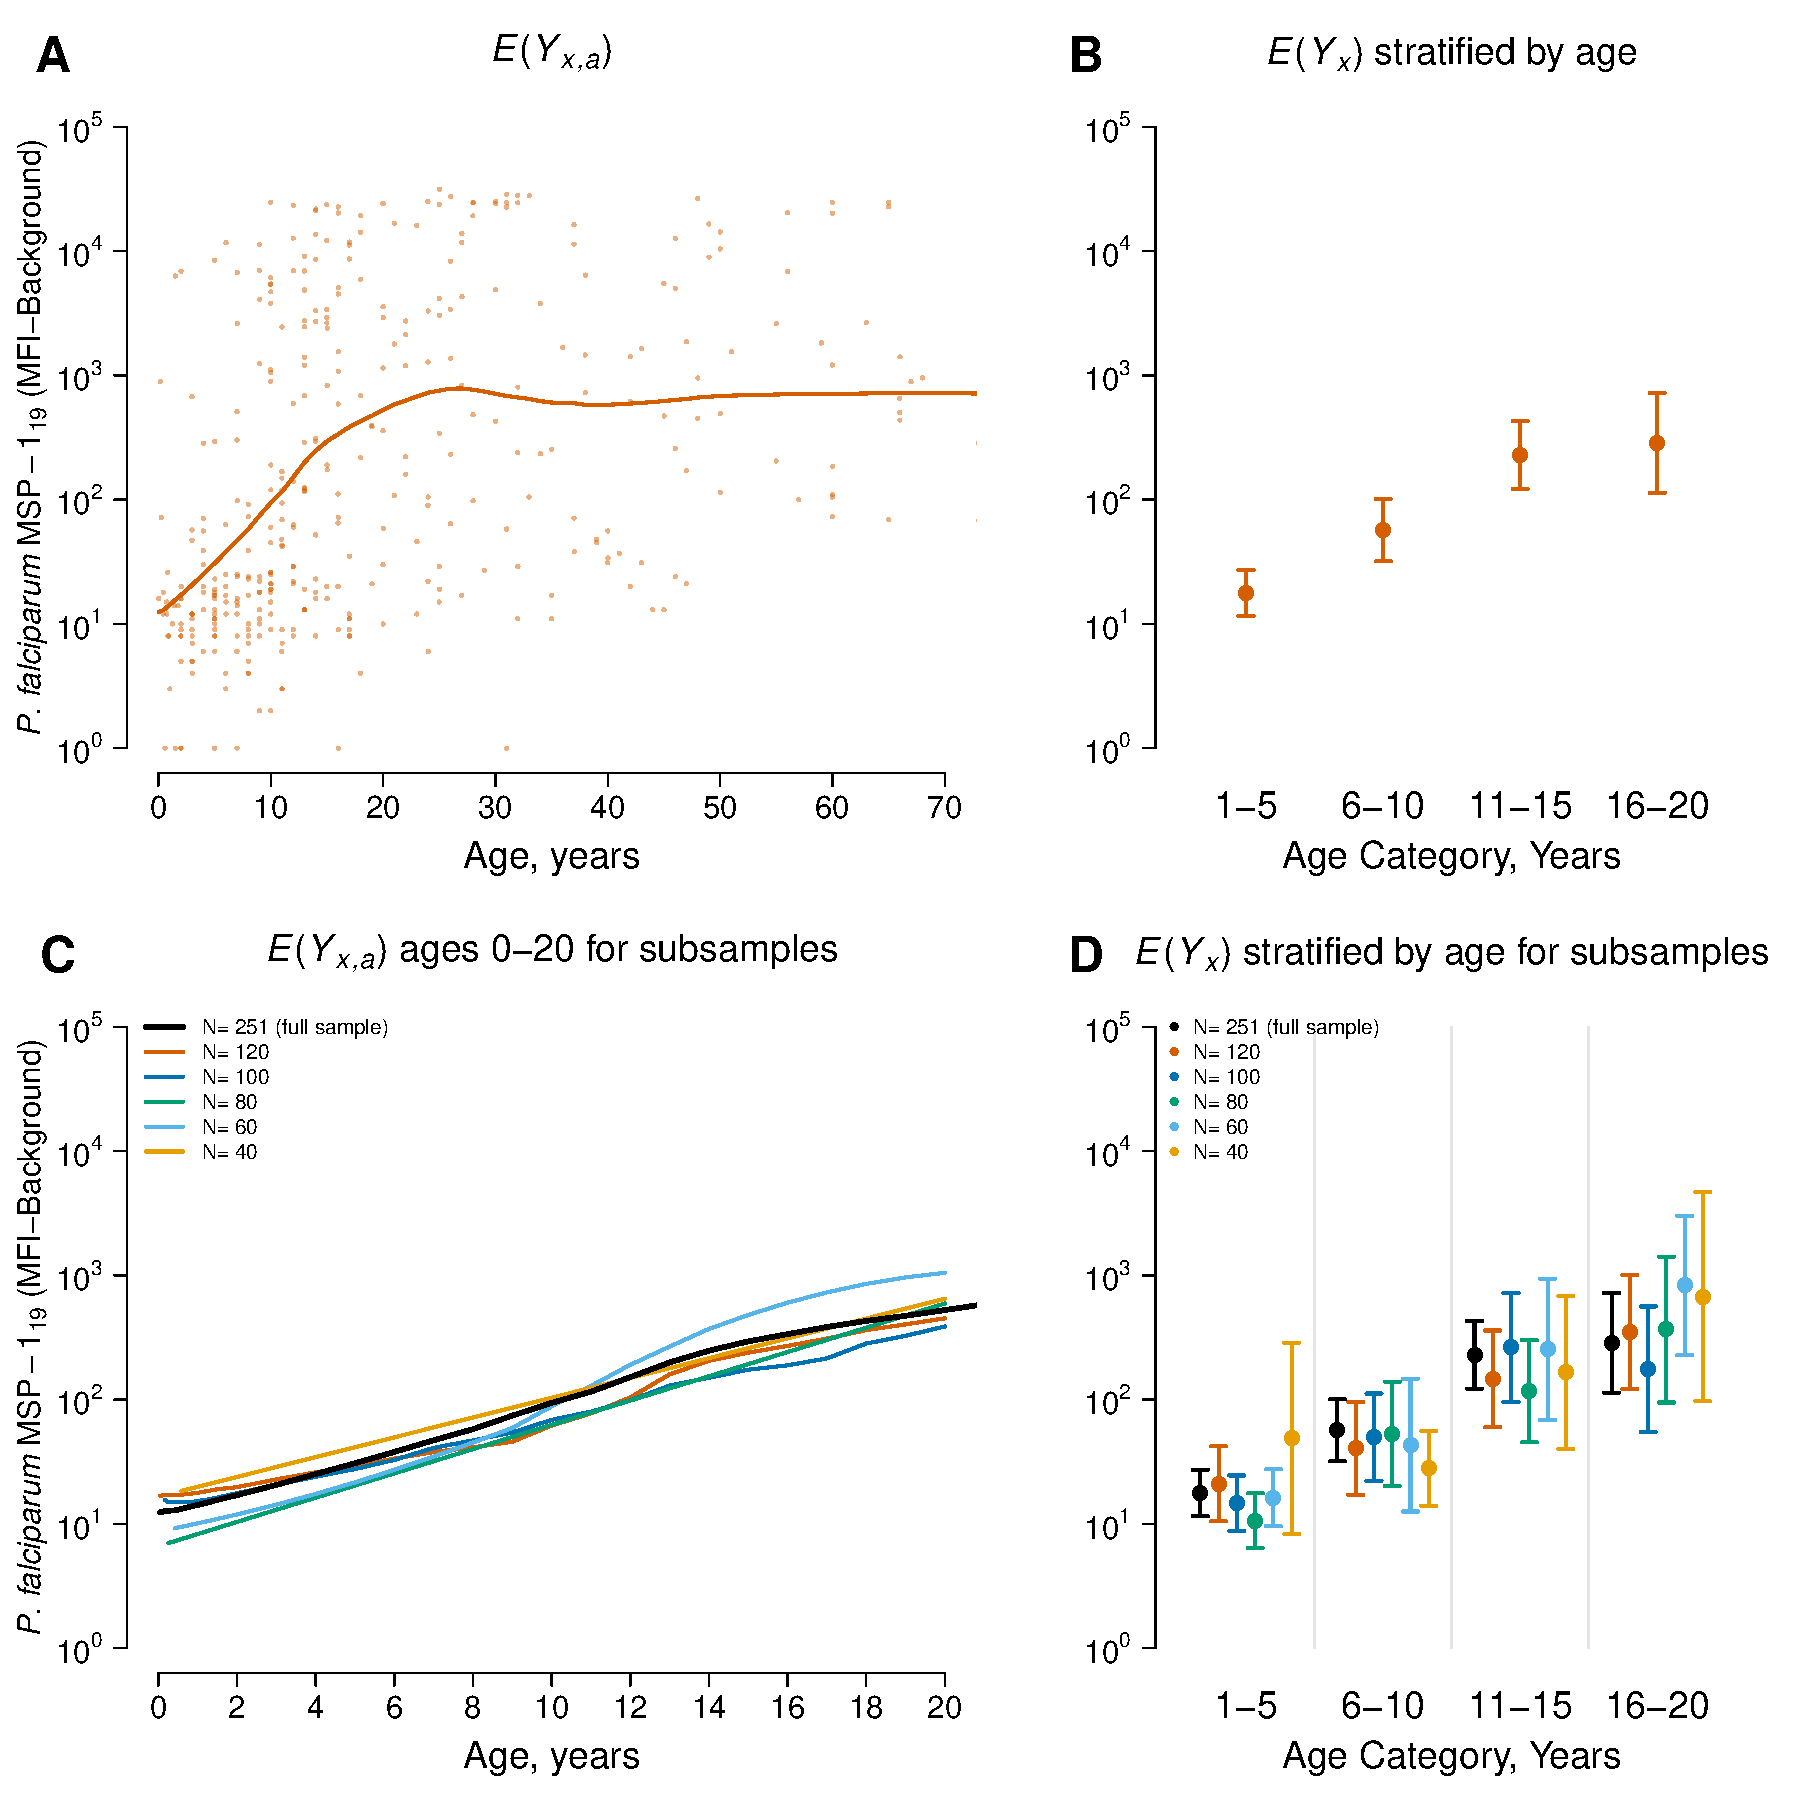
\includegraphics[width=\textwidth]{/users/benarnold/dropbox/articles/antibody-curves/results/figs/miton-msp1-analysis.pdf}
\begin{minipage}{\textwidth}
\caption{Age-antibody curve for IgG antibody response to the \textit{Plasmodium falciparum} merozoite surface protein-$1_{19}$ (MSP-$1_{19}$) antigen in a 1998 cross-sectional measurement of 383 individuals in the community of Miton, Haiti $^{23}$. A recombinant GST/MSP-$1_{19}$ fusion protein cloned from the \textit{P. falciparum} isolate 3D7 was included in a multiplex bead assay on the Luminex platform. (\textbf{a}) Mean antibody levels $E(Y_{a,x})$ by age ($a$) for ages 0-70 years; individual antibody responses (points) are shown along with a summary curve fit with an ensemble machine learning algorithm (Online Methods). (\textbf{b}) Age-adjusted geometric mean antibody response $E(Y_{x})$ and 95\% confidence intervals stratified by 5 year age category estimated using targeted minimum loss-based estimation (Online Methods). The number of individuals in each age group was: 1-5 (N=69), 6-10 (N=74), 11-15 (N=68), and 16-20 (N=40). In this example there is no stratification by group ($x$), but we have left the notation unchanged from other examples to make clear the comparison with other examples in the paper, such as Fig 3.}
\label{fig:mitonEYxa}
\end{minipage}
\end{center}
\end{figure}

%-------------------------------------------------------------------------------------------
% Figure S3 - Mauke results
%-------------------------------------------------------------------------------------------
\begin{figure}[htbp]
\begin{center}
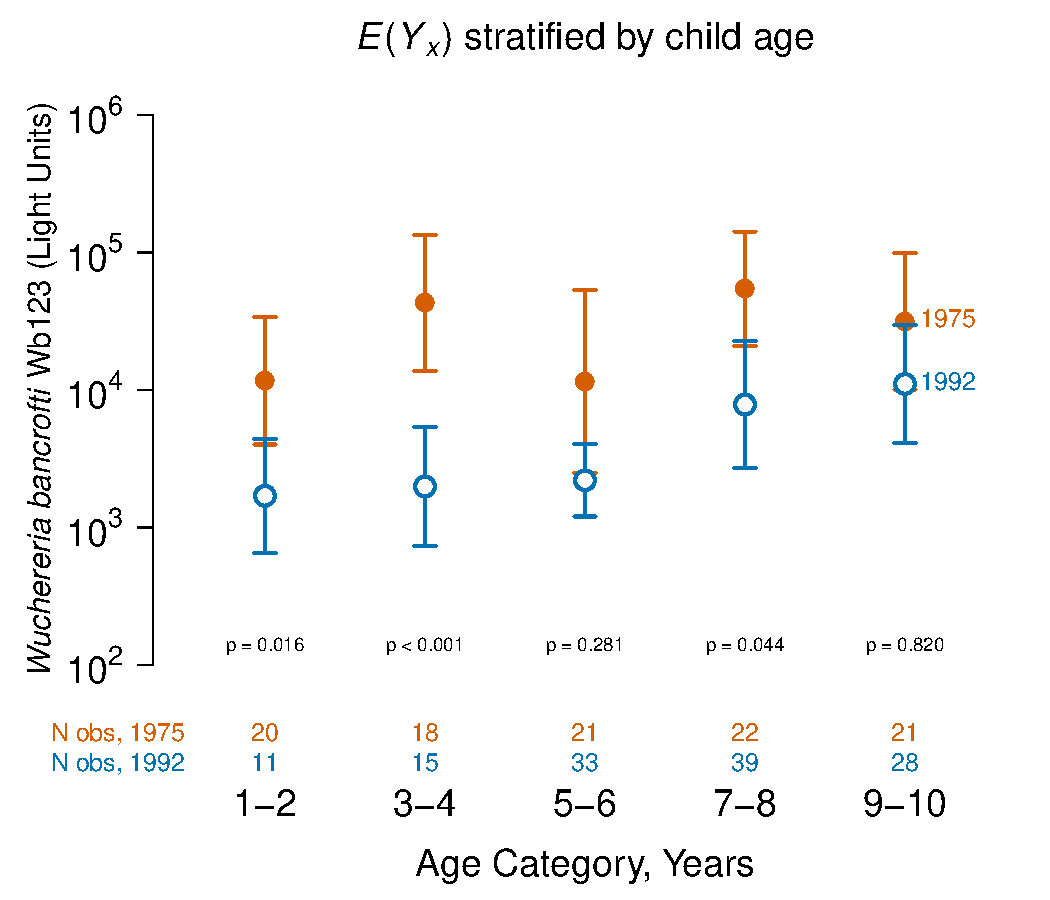
\includegraphics[width=0.75\textwidth]{/users/benarnold/dropbox/articles/antibody-curves/results/figs/mauke-Wb123-analysis-2y.pdf}
\begin{minipage}{0.75\textwidth}
\caption{Age-adjusted geometric mean antibody response $E(Y_{x})$ and 95\% confidence intervals to the Wb123 antigen for \textit{Wuchereria bancrofti} in 1975 and in 1992. The 1992 survey was five years after a single, island-wide mass drug administration (MDA) with diethylcarbamazine. The means are stratified by 2 year age band. The number of observations per stratum (N obs) is listed and $P$-values are Bonferroni-corrected tests of differences between means in each stratum.}
\label{fig:maukeS4}
\end{minipage}
\end{center}
\end{figure}


%-------------------------------------------------------------------------------------------
% Figure S4 - Mauke seroprevalence curves
%-------------------------------------------------------------------------------------------
\clearpage
\begin{figure}[htbp]
\begin{center}
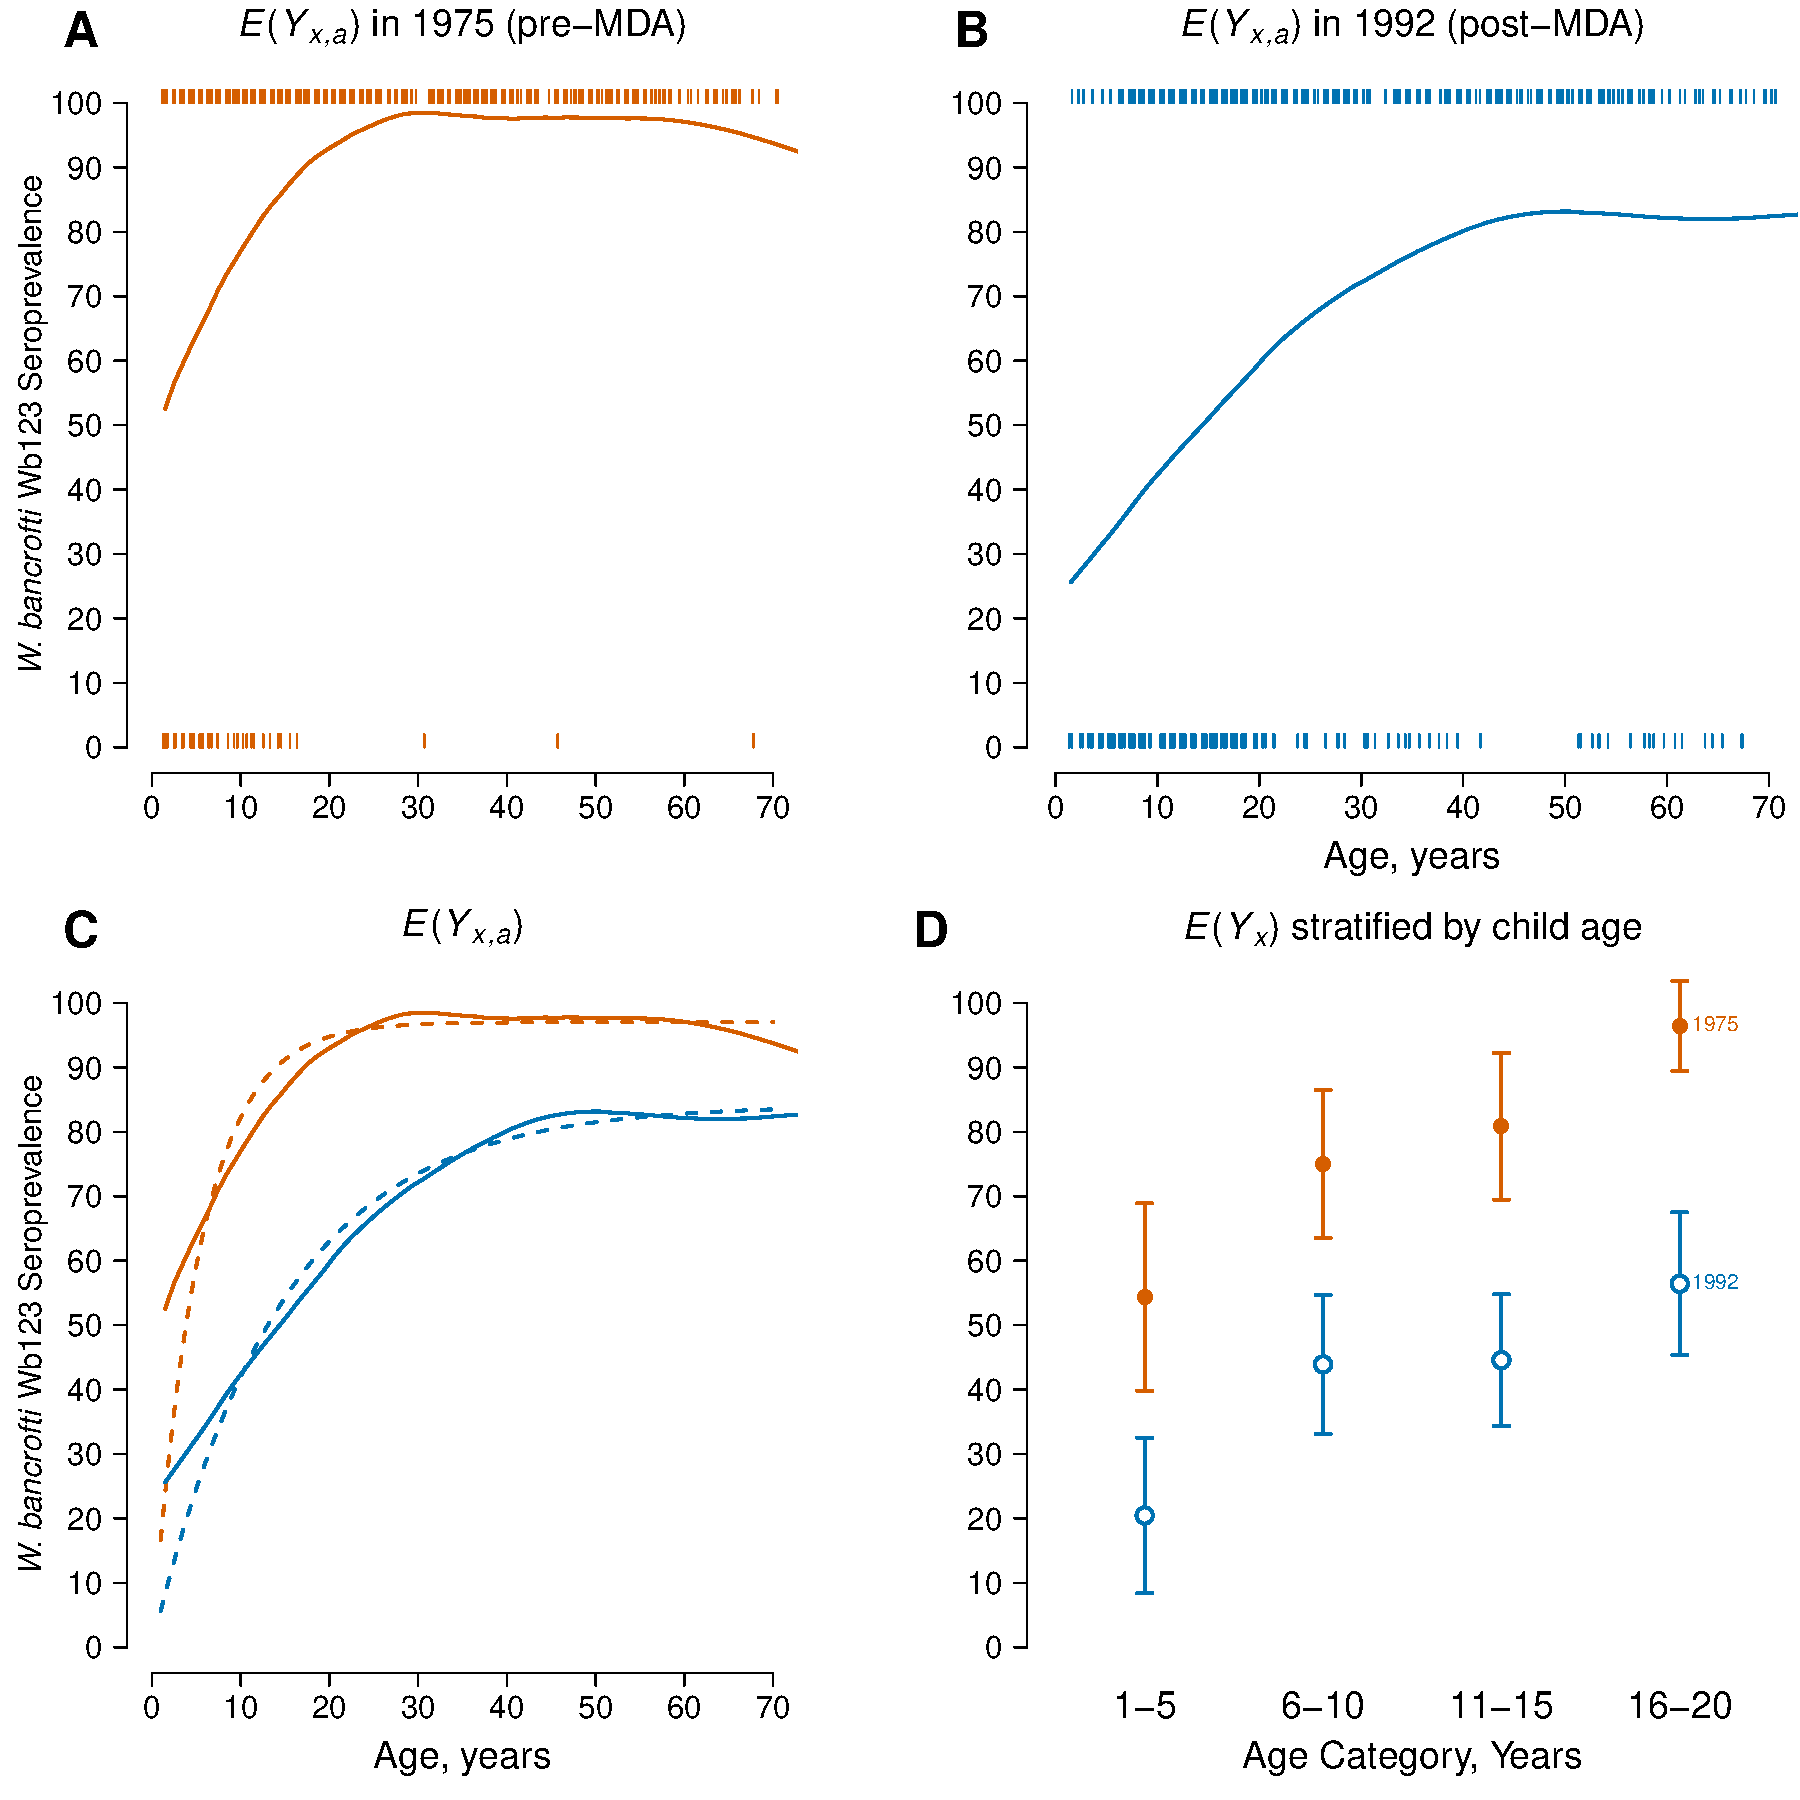
\includegraphics[width=\textwidth]{/users/benarnold/dropbox/articles/antibody-curves/results/figs/mauke-Wb123-binary.pdf}
\begin{minipage}{\textwidth}
\caption{Application of the methodology to binary (seropositive / seronegative) antibody measurements, typical of rapid diagnostic test results. Age-antibody curves illustrate a shift in transmission intensity of \textit{Wuchereria bancrofti} due to mass drug administration (MDA) on Mauke Island.  This figure presents a re-analysis of the results in main text Fig 3, but the quantitative antibody levels were reduced to seropositive and seronegative status using a previously determined cutoff value of 10968 with sensitivity >98\% and specificity >89\%.$^{53}$ Age-specific seroprevalence curves $E(Y_{a,x})$ in 1975 (\textbf{a}) and 1992 (\textbf{b}); rug plots include individual data points and summary curves were fit with a nonparametric ensemble machine learning algorithm (Online Methods). \textbf{c}, overlay of the curves in the two survey years to illustrate the shift due to lower transmission.  \textbf{d}, age-adjusted seroprevalence $E(Y_{x})$ and 95\% confidence intervals before (1975) and five years after (1992) MDA, stratified by 5 year age category (all differences significant at $P\leq0.01$ after Bonferroni correction).}
\label{fig:maukebina}
\end{minipage}
\end{center}
\end{figure}





\end{document}